\documentclass[18pt]{beamer}
\usepackage{templates/beamerthemekit}
\titlelogo{empty_logo}

% \titleimage{my_intro}
\titleimage{KASCADE-img}

\title[\texorpdfstring{$\gamma$}{gamma}-ray search in air shower arrays]{Developing stacked-analysis methods for \texorpdfstring{$\gamma$}{gamma}-ray search in air
shower arrays}
\subtitle{DPG-19, Aachen}
\author[V.~Tokareva, A.~Haungs, D.~Kostunin]{
  V.~Tokareva, A.~Haungs, D.~Kostunin~\textbar~25-29 March 2019}

\institute{Institute for Nuclear Physics (IKP)}

\date{March 26, 2019}

% 0. Титульник (Serach for high-energy gamma-rays...) +
% 1. Мотивация: зачем нужно изуать высокоэнергетические гамма? +
% 2. HAWC-sources +
% 3-4. CARPET2 results
% 5. KASCADE data: Efficiency of registretion, exposure map *
% 6. gamma/CR *
% 7. Предел на diffuse gamma flux (рез-ты Донгвы) +
% 8 - 10 Оценка количества событий вокруг 2HWC_J2013+415 +-
% 11. Присоединение данных TAIGA (Tunka-133, HiSCORE) (как идея)
%         отличие тунки от каскада, черенки/сцинтиляторы
%         картинки с хмах
%         мэппинг данных
%
%         разделение гамма/кр тунка133 +
% 12. Conclusion and future work
%
% Bonus slides:
% 13. data rates +
% 14. KCDC +
% 15. ML/DL opportunities +
% 16. GRADLC initiative +

% Bibliography
% \usepackage{textcomp}
\usepackage[citestyle=authoryear,bibstyle=numeric,hyperref,backend=biber]{biblatex}
\addbibresource{templates/example.bib}
\bibhang1em

\setbeamertemplate{navigation symbols}{}
\setbeamercovered{invisible}
\usepackage{tikz}
\newcommand{\itemarrow}{\scriptsize\raise1.25pt\hbox{\textcolor{kit-green100}{$\blacktriangleright$}}}
% \newcommand{\itemarrow}{\scriptsize\raise1.25pt\hbox{\textcolor{kit-blue30}{$\blacktriangleright$}}}
\newcommand{\concl}[1]{\item[\itemarrow]\textcolor{kit-green100}{#1}}
\renewcommand{\emph}[1]{\textcolor{kit-green100}{\textbf{#1}}}
\renewcommand{\thefootnote}{\fnsymbol{footnote}}
\newlength{\cellwidth}
\setlength{\cellwidth}{0.43\textwidth}
\newcommand{\cellbox}[1]{\parbox{\cellwidth}{\vspace{1ex}#1\vspace{1ex}}}
\newcommand{\insimg}[1]{
\begin{tikzpicture}[remember picture,overlay]
  \node[xshift=-7.7ex,yshift=12ex] at (current page.south east){%
    \includegraphics[width=14ex]{pics/#1}
  };
\end{tikzpicture}
}

\begin{document}
\selectlanguage{english}

%INTRODUCTION

%title page
\begin{frame}
\titlepage
\end{frame}

\section{High-energy \texorpdfstring{$\gamma$}{gamma} sources}

\begin{frame}{Why to study?}
  \begin{itemize}
    \item $\gamma$-rays:
    \begin{itemize}
        \item are not deflected by interstellar magnetic fields $\Rightarrow$ can be tracked to their origin;
        \item can be used for point sources search;
%         \item are able to provide answers about the Galactic cosmic ray propagation;
        \item $\gamma$-ray flux study could bring us insights on cosmic rays acceleration mechanisms.
    \end{itemize}
    \item UHE $\gamma$-rays (above $\sim50$~TeV):
    \begin{itemize}
        \item not so well-investigated because of flux intensity decrease for all CR particles at higher energies and because of a large absortion on the cosmic microwave background and interstellar matter;
        \item are supposed to be produced by black holes, neutron stars, supernova remnants, super-bubbles / star-forming regions / young massive star clusters;
        \item could improve our understanding about properties of matter in extreme states that cannot be studied in laboratories.
    \end{itemize}
  \end{itemize}
\end{frame}

%OURS SO FAR
%KASCADE gamma search

% \begin{frame}{KASCADE-Grande}
% \begin{itemize}
%   \item Proposed in 1989---disassembled in 2013;
%   \item Aimed at studying
%   high-evergy (galactic) cosmic rays by observing extensive air showers (EAS);
% %   processes at the edge of the Galaxy and beyond by observing extended atmospheric showers (EAS);
%   \item Consisted of:
%   \begin{itemize}
%     \item scintillators detecting $e$, $\gamma$, $\mu$:
%     \begin{itemize}
%   %сцинтиляторы, различают e, gamma, mu
%     \item KASCADE---256 stations;
%     \item GRANDE---37 stations;
%     \end{itemize}
%  %один большой калориметр
%     \item Hadronic callorimeter;
%  %радиодетектор
%     \item Digital radio array LOPES detecting $e$, $e^{+}$;
% % позволяющих наблюдать различные компоненты ливня
%   \end{itemize}
%   \item Important features of cosmic-ray spectrum have been obtained. The data analysis is ongoing;
% %  благодаря данным с эксперимента было открыто много всего ополезного, при этом анлиз данных продолжается. новые статьи выходят
%   \item KCDC (\textbf{K}ASCADE \textbf{C}osmic Ray \textbf{D}ata \textbf{C}enter, \textcolor{blue}{\texttt{http://kcdc.ikp.kit.edu}}) is a dedicated portal where all the data collected are available online. % At the moment
% \end{itemize}
% 
% \begin{frame}{KASCADE-Grande gamma-ray limits}
% %   \item Limits on the ratio of diffuse gamma-ray flux to cosmic ray flux
%   \begin{minipage}{0.5\textwidth}
%    left
%   \end{minipage}
% 
% %   \begin{columns}
% %     \column{0.5\textwidth}
% %     left
% %     \column{0.5\textwidth}
% %     right
% %   \end{columns}
% \end{frame}


\section{KASCADE high-energy \texorpdfstring{$\gamma$}{gamma}-ray search}

\begin{frame}{High-energy $\gamma$-ray sources in KASCADE field of view}
%   KASCADE data: Efficiency of registration, exposure map *
  
  \begin{center}
    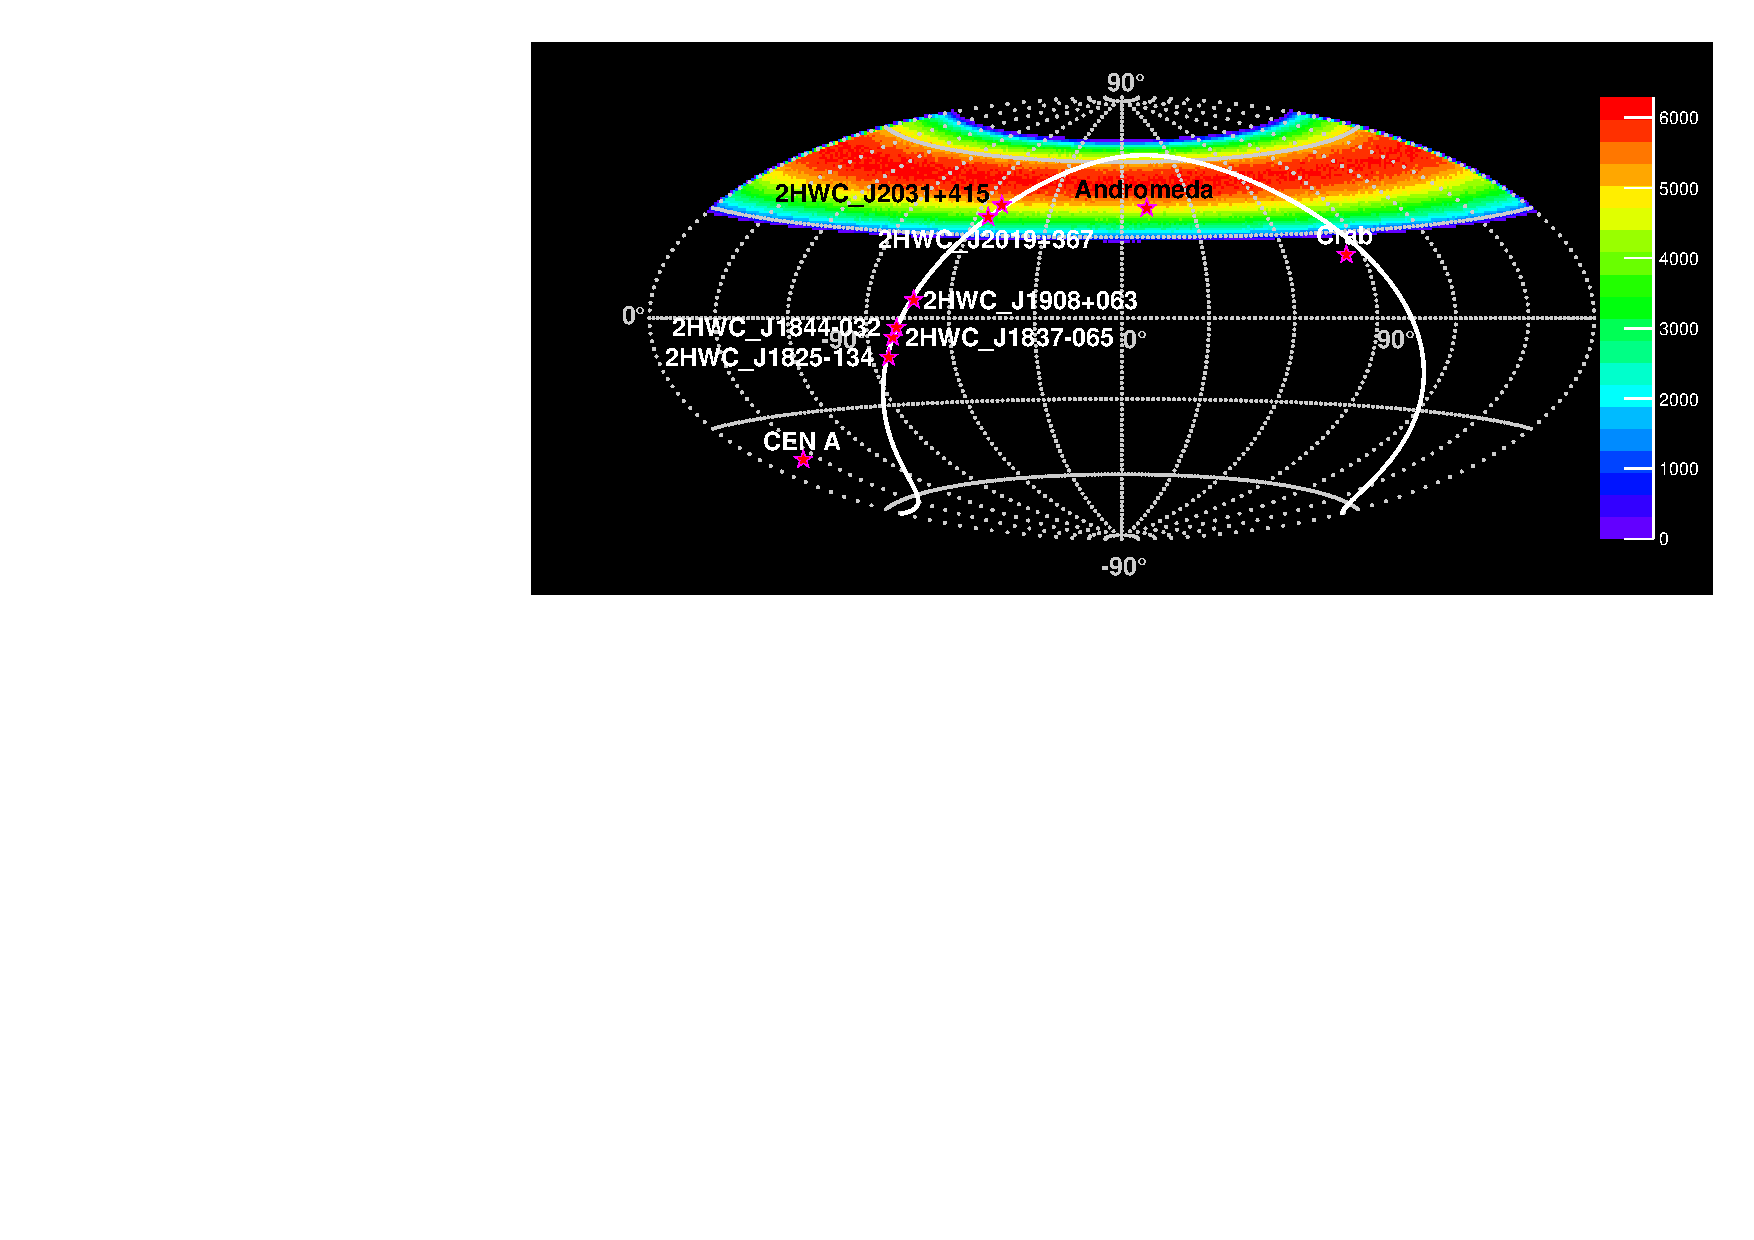
\includegraphics[width=1\textwidth]{pics/Skymap_6srcs.pdf}
    
 KASCADE events distribution map
  with 6 HAWC sources with energy \\$E$ above 56 TeV and galactic center and anti-center.
\end{center}
\end{frame}

\begin{frame}{KASCADE-Grande $\gamma$ ray searches}
\begin{itemize}
 \item Limits on the ratio of diffuse gamma-ray flux to cosmic ray flux
\end{itemize}

\begin{center}
    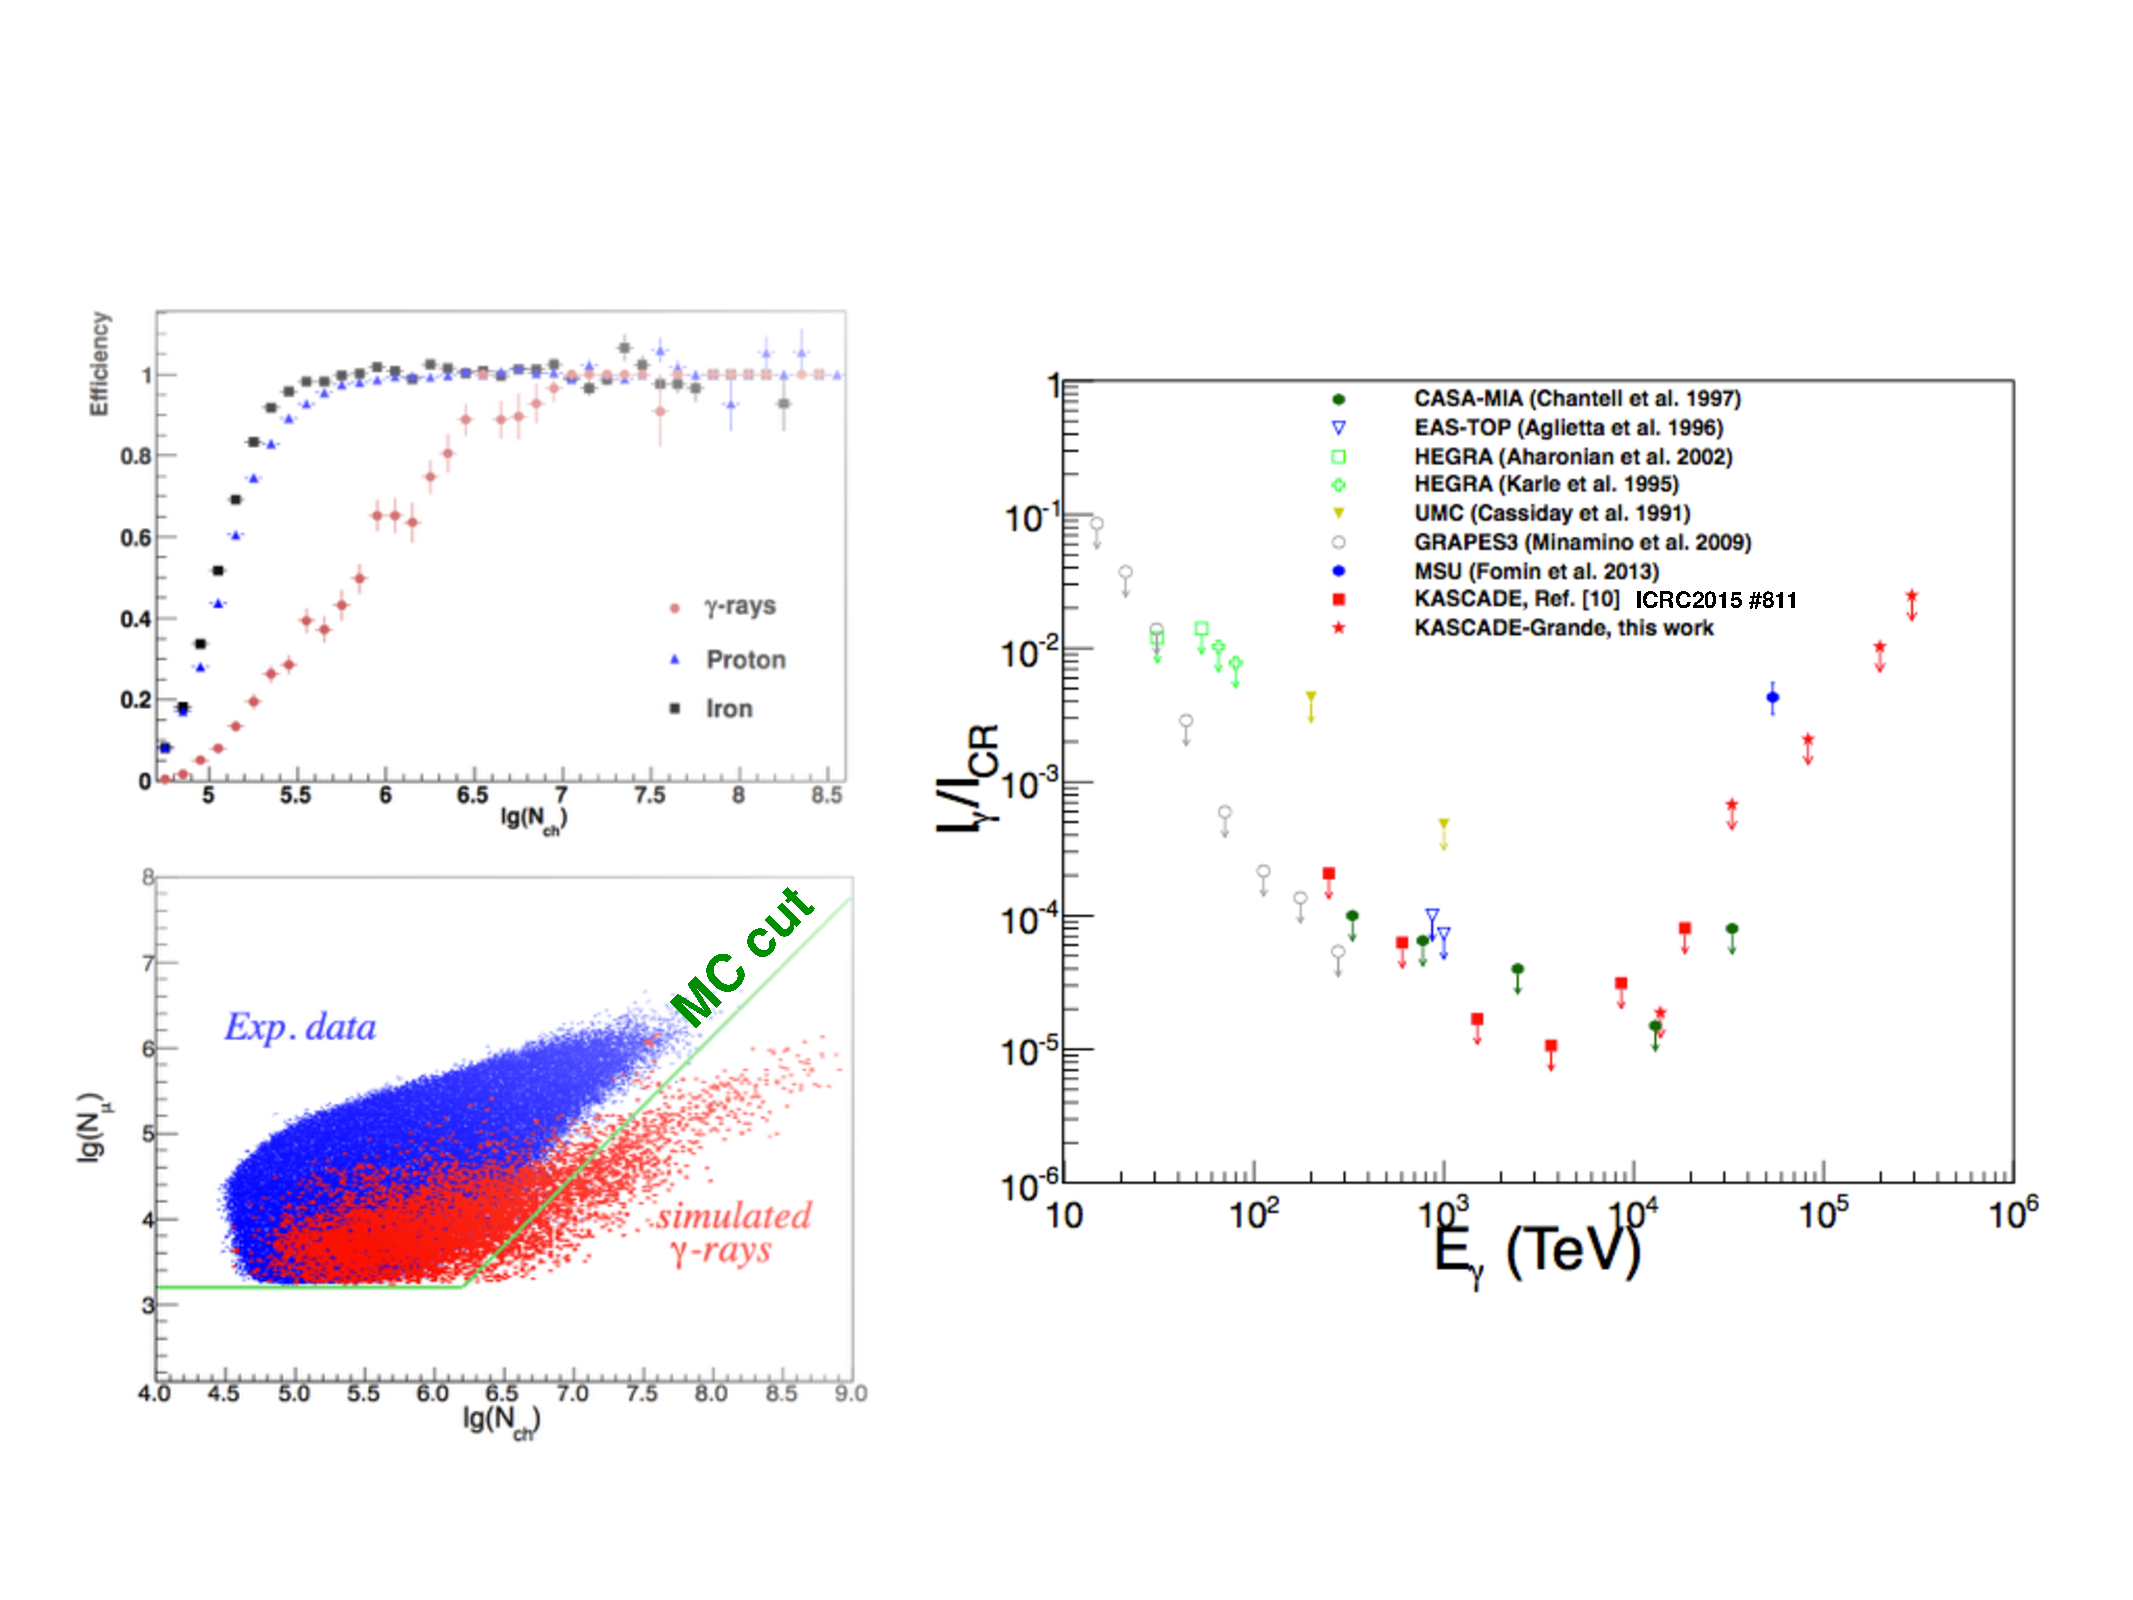
\includegraphics[width=0.90\textwidth]{pics/KASCADE-Grande_UHECR2016.pdf}
\end{center}
\end{frame}

\begin{frame}{KASCADE-Grande $\gamma$ ray searches}
\begin{itemize}
 \item Limits on the diffuse gamma-ray flux: the best upper limit of the fraction of $\gamma$-rays
to the total cosmic ray flux is obtained at $3.7 \times 10^{15}$~eV with $1.1 \times 10^{-5}$. 
\end{itemize}

\begin{center}
    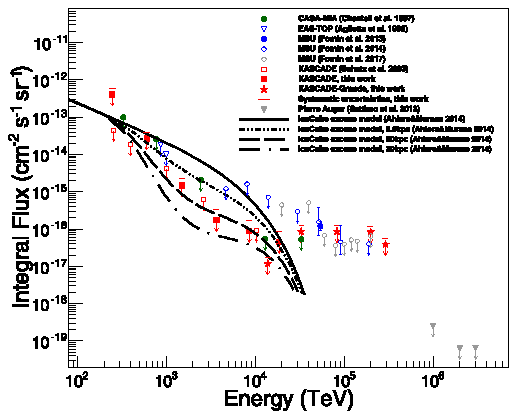
\includegraphics[width=0.57\textwidth]{pics/KASCADE-Grande_UHECR2016-2.pdf}
\end{center}
\end{frame}

\begin{frame}{$\gamma$-proton separation}
\small
% \begin{figure}[h]
\vspace{-1em}
\begin{center}
    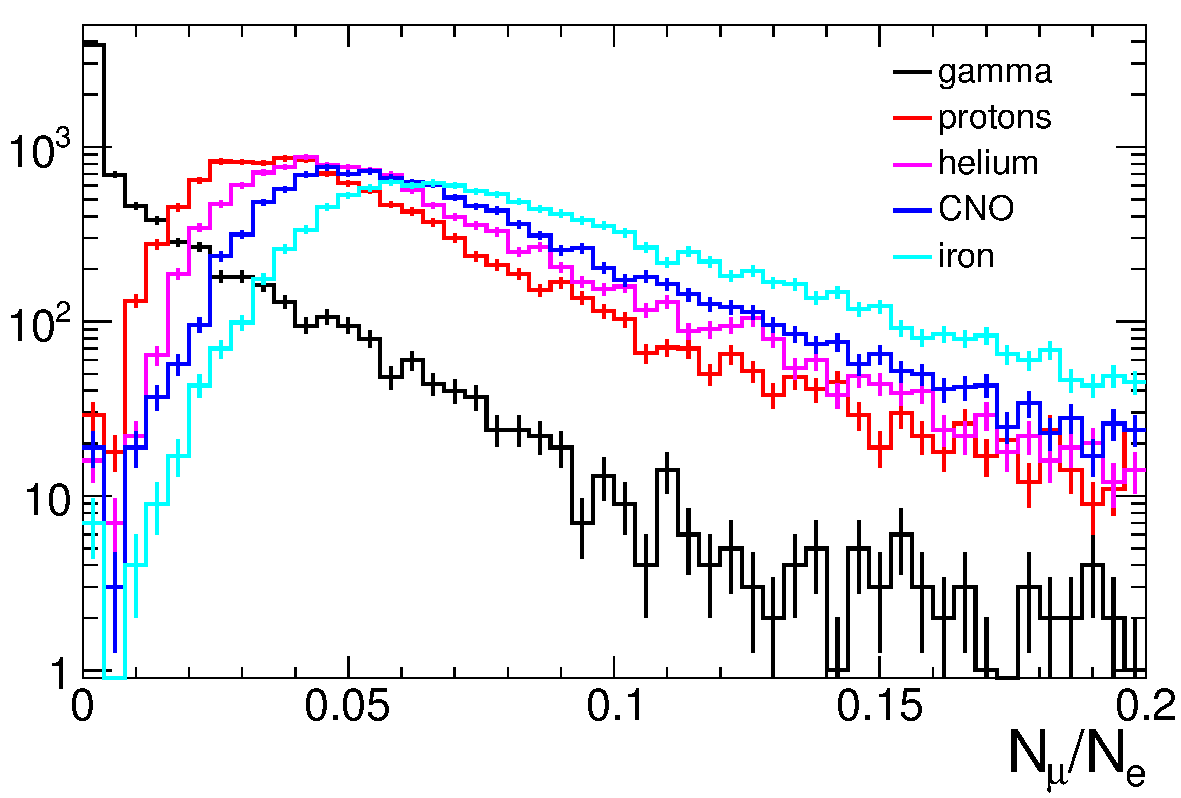
\includegraphics[width=0.65\textwidth]{pics/Nmu_Ne.pdf}
    
    Distribution of $N_\mu / N_e$ for various primary CR components.
\end{center}
%   Распределение компонент ливня в зависимости от соотношения мюоной и электронной компоненты ливня
% \caption{
% \vspace{1em}
% }
%  \end{figure}
Taking into account this distribution and the flux upper-limit mentioned above we can make the 
$N_\mu/N_e \in [0, 0.008)$ cut to discriminate $\gamma$ component with ... C.L.
\end{frame}

\begin{frame}{HAWC high-energy sources in KASCADE field of view}
 \begin{center}
    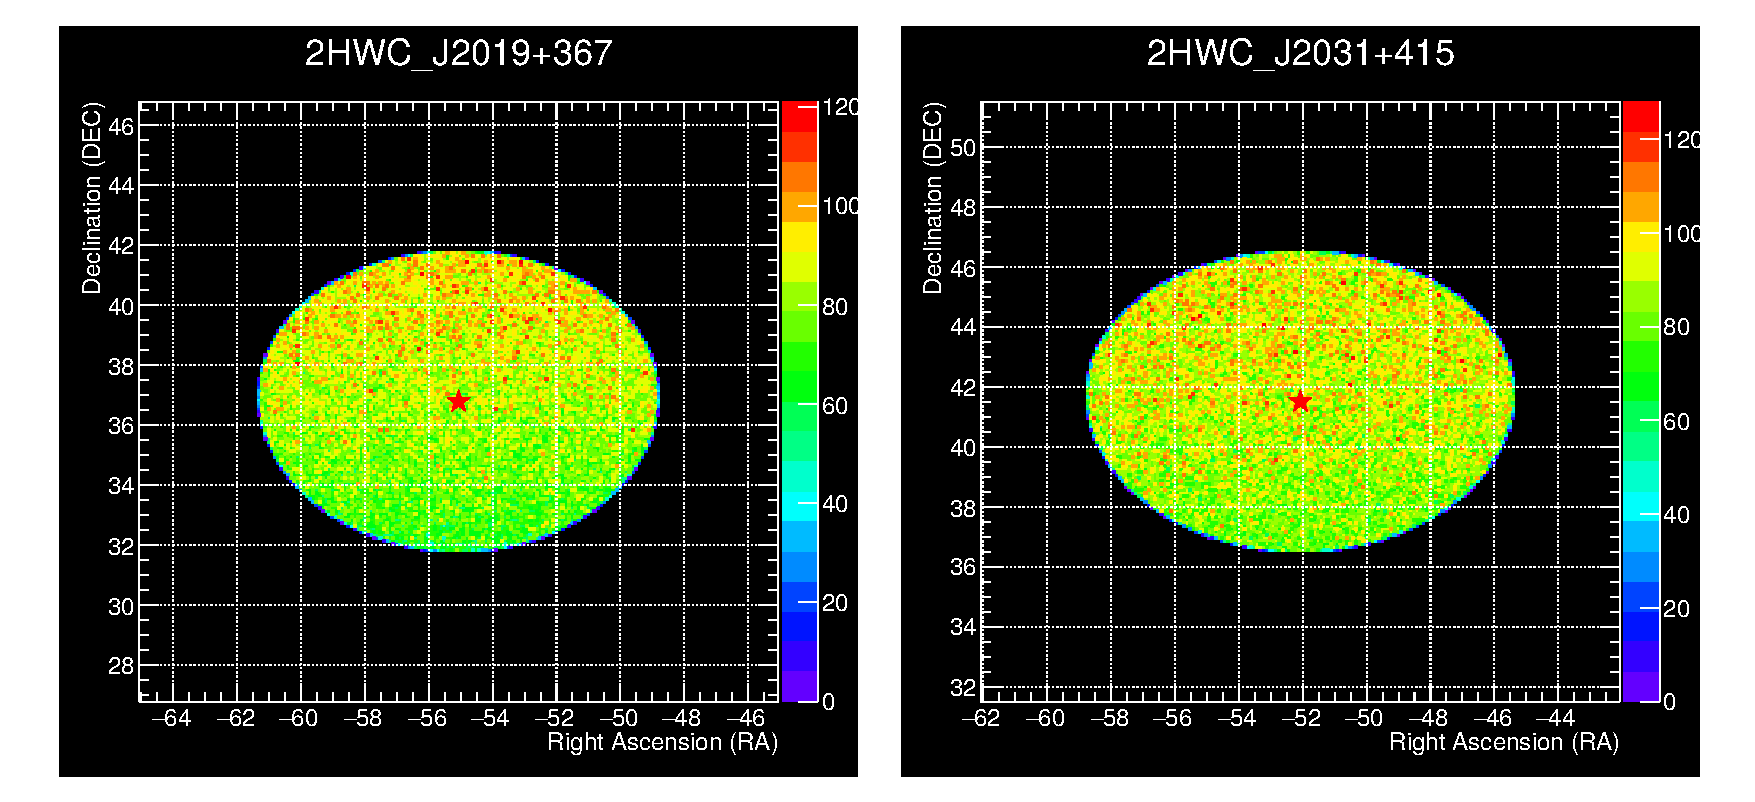
\includegraphics[width=1\textwidth]{pics/2HWCsources.pdf}
    
 Events by KASCADE in $5^0$ radius around the point sources $2HWC_J2019+367$, $2HWC_J2031+415$ correspondingly.

\end{center}
\end{frame}


\begin{frame}{KASCADE statistics estimation for $2HWC_J2013+415$}

\begin{table}[]
\begin{tabular}{lll}
E &       N &      $F_{int}$  \\
7 & 440.9659202598506 & 1.406167411764706e-13\\
56 & 12.857367242057173 & 4.100001833751227e-15\\
100 & 4.798126510222744 & 1.5300432133675341e-15\\
1000 & 0.09573521008300581 & 3.052837563906128e-17\\
\end{tabular}
\end{table}

% There supposed to be 2 slides on this
%  Оценка количества событий вокруг 2HWC_J2013+415 +-
\end{frame}

%Tunka133
%adding TAIGA|Tunka data

% 11. Присоединение данных TAIGA (Tunka-133, HiSCORE) (как идея)
%         отличие тунки от каскада, черенки/сцинтиляторы
%         картинки с хмах
%         мэппинг данных
%
%         разделение гамма/кр тунка133 +

\begin{frame}{KASCADE-TAIGA joint analysis}
 Why possible?
\end{frame}

\begin{frame}{Tunka-133 $\gamma$ - proton separation}
    \begin{center}
	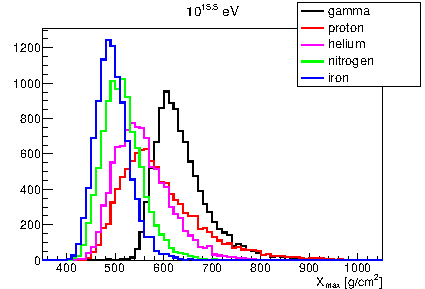
\includegraphics[width=0.8\textwidth]{pics/tunka_gamma_cr_diff.pdf}
	
      Distribution of $X_{max}$ for various primaries at $E = 10^{5.5} eV$.
    \end{center}
\end{frame}


% %CONCLUSION
\section{Conclusion}

% \begin{frame}{Open access and education}
%     \vspace{-4em}
%     \begin{itemize}
%         \item Open access: a dedicated portal planned
%         \item Education: \textcolor{blue}{\texttt{astroparticle.online}}
%     \end{itemize}
%     \centering
%     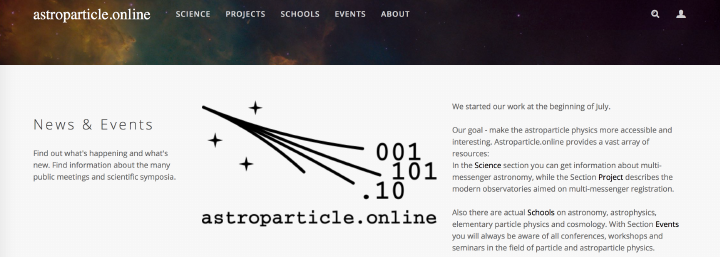
\includegraphics[width=0.85\textwidth]{pics/astro_onl.png}
% \end{frame}

\begin{frame}{Outlook}
% \textcolor{red}{Improve the translation quality!!!}
\begin{itemize}
\item Done so far:
    \begin{itemize}
    \item Metadata DB filled out with sample data of KASCADE and Tunka-133;
    \item The filling with the main amount is ongoing;
    \end{itemize}
\item ToDo: 
    \begin{itemize}
     \item Metadata extractor for KCDC;
    \end{itemize}

\item Open for discussion:
\begin{itemize}
 \item 2nd level MD search - the place in the general scheme;
 \item user interface;
 \item data mapping;
\end{itemize}

 \end{itemize}
\end{frame}

% \subsection{The end}
% \begin{frame}{}
%     \begin{center}
%         \textcolor{kit-green100}{\Huge Thank you\\for your attention!\vspace{1em}}  
%         \Large Any questions?
%     \end{center}
% \end{frame}


%BACKUP SLIDES
\appendix
\beginbackup
%bonus slides

% 13. data rates +
% 14. KCDC +
% 15. ML/DL opportunities +
% 16. GRADLC initiative +
\begin{frame}
 \huge
 \center
 Bonus slides
\end{frame}


%GRADLC initiative descripton 

\begin{frame}{German-Russian Astroparticle \\Data Life Cycle Initiative\footnotemark[1]}
\vspace{-1.4em}
\begin{center}
  
\includegraphics[width=0.9\textwidth]{pics/Collab-4.pdf}
\end{center}
\footnotesize\footnotetext[1]{Granted by RSF-Helmholtz Joint Research Groups}
\end{frame}

% %experiments overview

\begin{frame}{KASCADE-Grande}
\begin{itemize}
  \item Proposed in 1989---disassembled in 2013;
  \item Aimed at studying
  high-evergy (galactic) cosmic rays by observing extensive air showers (EAS);
%   processes at the edge of the Galaxy and beyond by observing extended atmospheric showers (EAS);
  \item Consisted of:
  \begin{itemize}
    \item scintillator arrays:
%     detecting $e$, $\gamma$, $\mu$:
    \begin{itemize}
  %сцинтиляторы, различают e, gamma, mu
    \item KASCADE---256 stations;
    \item GRANDE---37 stations;
    \end{itemize}
 %один большой калориметр
    \item Hadronic callorimeter;
 %радиодетектор
    \item Digital radio array LOPES;
%     detecting $e$, $e^{+}$;
% позволяющих наблюдать различные компоненты ливня
  \end{itemize}
  \item Important features of cosmic-ray spectrum have been obtained. The data analysis is ongoing;
%  благодаря данным с эксперимента было открыто много всего ополезного, при этом анлиз данных продолжается. новые статьи выходят
  \item KCDC (\textbf{K}ASCADE \textbf{C}osmic Ray \textbf{D}ata \textbf{C}enter, \textcolor{blue}{\texttt{http://kcdc.ikp.kit.edu}}) is a dedicated portal where all the data collected are available online. % At the moment
\end{itemize}

\begin{tikzpicture}[remember picture,overlay]
  \node[xshift=-12ex,yshift=-21ex] at (current page.north east){%
    
\includegraphics[width=0.3\textwidth]{pics/KCDC-Logo.png}
  };
\end{tikzpicture}
% \parbox[t][0pt]{0pt}{
%   \vspace{-0.63\textheight}
%   ~\hspace{0.68\textwidth}
\includegraphics[width=0.3\textwidth]{pics/KCDC-Logo.png}
% }
\end{frame}

\begin{frame}{TAIGA - Tunka Advanced Instrument for cosmic ray physics and Gamma Astronomy}
% \footnotesize
% % \vspace{-1em}
\begin{itemize}
 \item The detectors construction started in 90s with Tunka-25 setup;
 \item Changed name from Tunka to TAIGA;
 \item Is ongoing and continiously enhancend;
%  \item Currently consists of 4 detectors presented + TUNKA IACT is under construction;
\end{itemize}

% \vspace{2em}

\begin{center}
    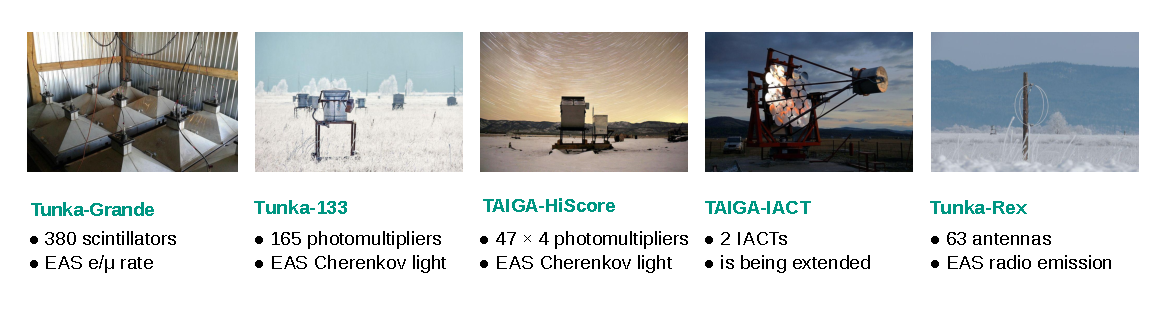
\includegraphics[width=1\textwidth]{pics/TAIGA_exp_wt.pdf} 
\end{center}

\end{frame}

 - experiments overview. Is not requiered is this IT=specified presentation
% 
% \begin{frame}{The main objectives}
% \begin{minipage}[c]{0.45\textwidth}
%   \begin{itemize}
%     \item  Provide sustainable access to scientific data
%     \item  Archiving of Data and Metadata
%     \item  Providing analysis tools
%     \item  Education in Big Data Science
%   \end{itemize}
% \end{minipage}
% \hfill
% \begin{minipage}[c]{0.54\textwidth}
%   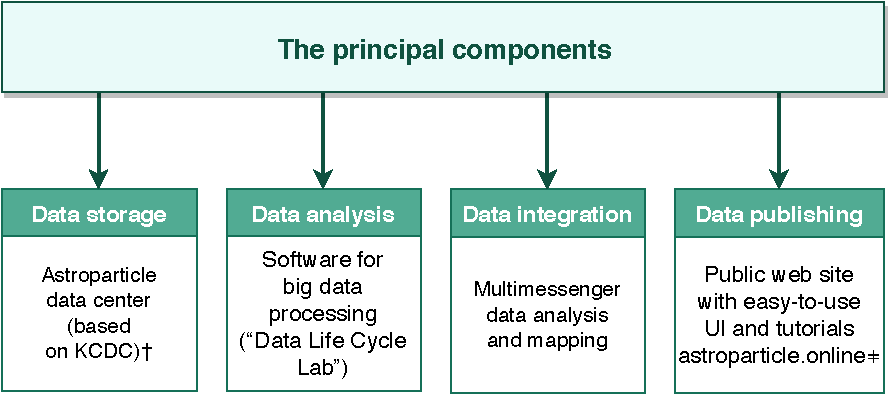
\includegraphics[width=1\textwidth]{pics/proj_objectives.pdf}
% \end{minipage}
%   \vspace{-\topsep}
%   \vspace{-\partopsep}
%   \vspace{\itemsep}
%   \vspace{\parsep}
%   \begin{itemize}
%     \item  Development area for multi-messenger analyses (e.g. Deep Learning)
%     \item  Platform for communication and exchange within Astroparticle Physics
%   \end{itemize}
% \end{frame}
% 


\begin{frame}{KASCADE Cosmic-ray Data Center (KCDC)}
    \begin{itemize}
        \small
        \setlength{\itemsep}{0pt}
        \item providing free, unlimited, reliable open access to KASCADE cosmic ray data at \textcolor{blue}{\underline{https://kcdc.ikp.kit.edu}};
        \item almost all KASCADE data is available;
        \item selection of fully calibrated quantities and detector signals;
        \item information platform: physics and experiment backgrounds, tutorials, meta information for data analysis;
        \item archive of KASCADE software and data;
        \item uses modern and open source web technologies.
    \end{itemize}


\includegraphics[height=0.35\textheight]{pics/KCDC-Logo.png}
\hfill
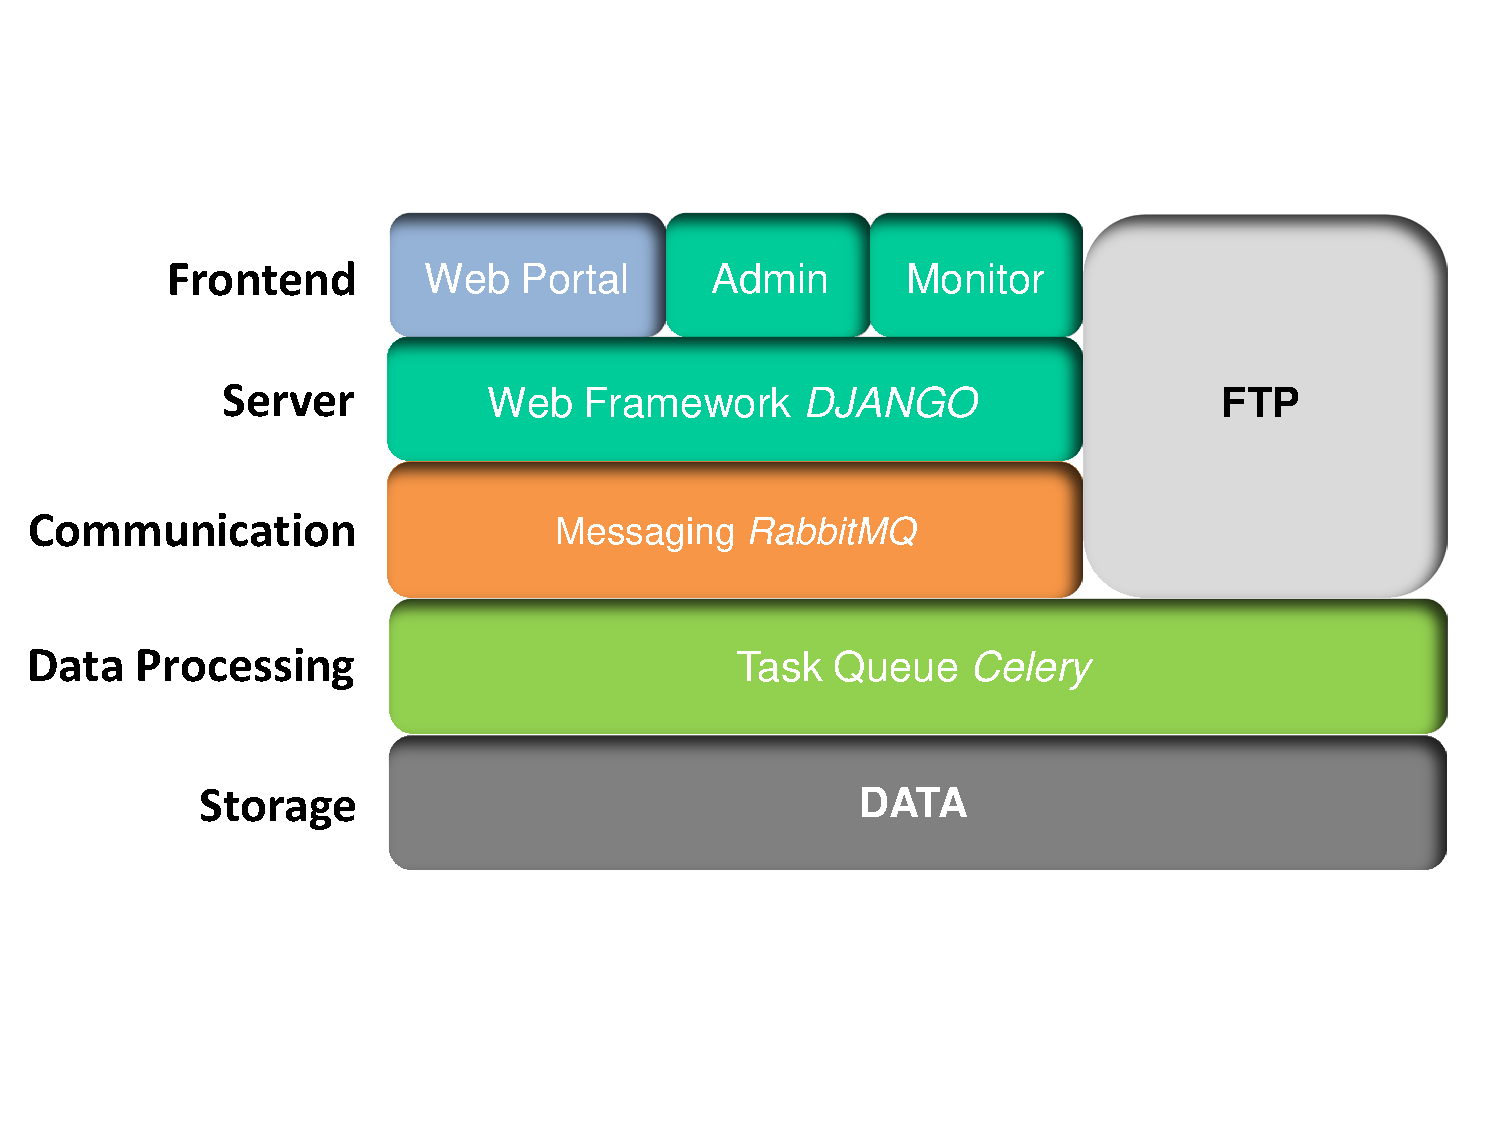
\includegraphics[height=0.35\textheight]{pics/KCDC-IT-Structure.pdf}
\end{frame}

\begin{frame}{KASCADE and TAIGA data rates}
\begin{minipage}[c]{0.52\textwidth}
% \small
  \begin{itemize}
    \item KASCADE:
    \begin{itemize}
      \item 450 000 000 events
      \item $\sim 4$~TB of measured data
    \end{itemize}
    \vspace{1em}
    \item planned TAIGA rate: $\sim 20$~TB/year
    \begin{itemize}
      \item HiSCORE: $\sim 18$~TB/year
      \item IACT: $\sim 1.5$~TB/year
      \item others: $\sim 0.5$~TB/year
    \end{itemize}
  \end{itemize}
\end{minipage}
\hfill
\begin{minipage}[c]{0.47\textwidth}
\vspace{-3.5em}
  \begin{itemize}
    \item current TAIGA rate: 
    \begin{itemize}
      \item $\sim 50$~Tb of raw data;
      \item $\sim 8$~TB/year of reconstructed data:
      \begin{itemize}
	\item HiSCORE: $\sim 6.4$~TB/year
	\item IACT: $\sim 1$~TB/year
	\item others: $\sim 0.5$~TB/year
      \end{itemize}
    \end{itemize}
  \end{itemize}
\end{minipage}

\end{frame}

\begin{frame}{Machine and deep learning opporutities}
 \begin{itemize}
  \item Search for anisotropies --- Clasterization;
  \item Distinguishing gamma/not gamma (distribution-based [$\beta$]) --- Classification.
 \end{itemize}

\end{frame}

%Appendix: detailed information on collaboration and links to the main sources

% \appendix
% \beginbackup
\section{Appendix}
\subsection{Collaboration}
\begin{frame}[allowframebreaks]
{The German-Russian Astroparticle Data Life Cycle collaboration}
\parbox{0.35\textwidth}{
  \centering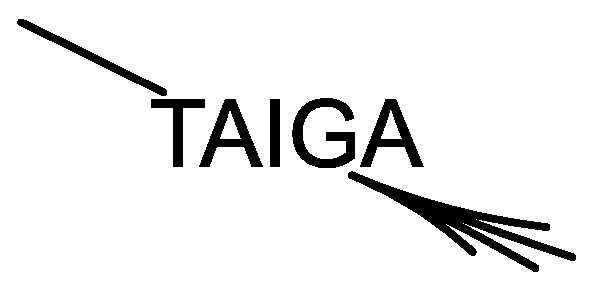
\includegraphics[width=0.25\textwidth]{pics/taiga.eps}
}\hfill
\parbox{0.60\textwidth}{
  TAIGA---Tunka Advanced Instrument for cosmic ray physics and Gamma Astronomy (see
%       https://
  taiga-experiment.info);
}
\\\vspace{1em}
\parbox{0.35\textwidth}{
  \centering
\includegraphics[width=0.35\textwidth]{pics/grande.pdf}
}\hfill
\parbox{0.60\textwidth}{
  KASCADE-Grande---KArlsruhe Shower Core and Array DEtector---Grande\\ (see
%       http://
  www-ik.fzk.de/KASCADE\_home.html);
}
\\\vspace{1em}
\parbox{0.35\textwidth}{
  \centering
\includegraphics[width=0.30\textwidth]{pics/Logo_KIT_IKP.pdf}
}\hfill
\parbox{0.60\textwidth}{
  KIT-IKP---Institute for Nuclear Physics Karlsruhe Institute of Technology
}
\\\vspace{1em}
\parbox{0.35\textwidth}{
  \centering
\includegraphics[width=0.15\textwidth]{pics/SCC-Logo.png}
}\hfill
\parbox{0.60\textwidth}{
  SCC---Steinbuch Centre for Computing Karlsruhe Institute of Technology
}
\\\vspace{1em}
\parbox{0.20\textwidth}{
  \centering
\includegraphics[width=0.20\textwidth]{pics/SINP_MSU_LOGO.pdf}
}\hfill
\parbox{0.75\textwidth}{
  SINP MSU---Skobeltsyn Institute Of Nuclear Physics Lomonosov Moscow State University
}
\\\vspace{1em}
\parbox{0.20\textwidth}{
  \centering
\includegraphics[width=0.15\textwidth]{pics/isu_logo.png}
}\hfill
\parbox{0.75\textwidth}{
  ISU---Irkutsk State University
}
\\\vspace{1em}
\parbox{0.20\textwidth}{
  \centering
\includegraphics[width=0.18\textwidth]{pics/matr_logo.png}
}\hfill
\parbox{0.75\textwidth}{
  ISDCT---Matrosov Institute for System Dynamics and Control Theory
}
\end{frame}

\subsection{References}
    \begin{frame}{References}
        \begin{itemize}
            \item Berghöfer T., Agrafioti I. \textit{et al.} Towards a model for computing in European astroparticle physics,
            Astroparticle Physics European Coordination committee, 2016,
            web-source:~\texttt{http://appec.org/wp-content/uploads/\\Documents/Docs-from-old-site/AModelForComputing-2.pdf};
            \item KCDC---\textbf{K}ASCADE \textbf{C}osmic Ray \textbf{D}ata \textbf{C}enter,\\
            web-source:~\texttt{http://kcdc.ikp.kit.edu};
            \item KASCADE-Grande official site, web-source:~\texttt{http://www-ik.fzk.de/KASCADE\_home.html};
            \item TAIGA collaboration official site, web-source:~\texttt{http://taiga-experiment.info};
            \item Astroparticle.online---outreach resource, web-source:~\texttt{http://astroparticle.online}.
        \end{itemize}
    \end{frame}
% \backupend

\backupend
\end{document}
